%
% File naaclhlt2013.tex
%

\documentclass[11pt,letterpaper]{article}
\usepackage{naaclhlt2013}
\usepackage{times}
\usepackage{graphicx}
\usepackage{latexsym}
\usepackage{listings}
\usepackage{algorithmicx}
\lstset{
		basicstyle=\ttfamily\footnotesize,       % the size of the fonts that are used for the code
		numbers=left,                   % where to put the line-numbers
		numberblanklines=false
		numbersep=1em,                  % how far the line-numbers are from the code
		basewidth=0.52em,
		tabsize=4,  		% sets default tabsize to 2 spaces
		xleftmargin=\leftmargini
      }
\renewcommand*\thelstnumber{\the\value{lstnumber}:}
% END lstlisting environments

\lstnewenvironment{sql}[1][]{\lstset{language=SQL,gobble=4,emphstyle=\textit,#1}}{}


\setlength\titlebox{6.5cm}    % Expanding the titlebox

\title{Large-scale Statistical Text Analytics in Relational Databases\Thanks{This
    and NAACL proceedings, including those for 
    the {\em International Joint Conference on Artificial Intelligence}.  
    This second version clarifies the procedure for 
    submitting for double-blind reviewing.}}

\author{Kun Li, Christan Grant, Daisy Zhe Wang\\
	    University of Florida\\
	    111 Anywhere Street\\
	    Gainesville, FL 32608, USA\\
	    {\tt kli@cise.ufl.edu}
	  \And
	George Chitouras\\
  	Greenplum/EMC\\
  	900 Main Street\\
	    Gainesville, FL 32608, USA\\
  {\tt george.chitouras@emc.com}}

\date{}

\begin{document}
\maketitle
\begin{abstract}
  In this paper we introduce MADText a statistical text analytics module 
  contributed to MADLib which is an open source project for statistical and parallel library
  for in-database analytics.
  Instead of extracting text features on fly, we precomputed the text features.
  MADText can do part-of-speech tagging and entity detection. 
  We show that our package is linearly scalable and outperform the state of art packages.
  Lastly, we show we can our MADText to do near real time hot topics discovery over all the states of USA. 
  We can analyze 1 million tweets in 3 minutes using a machine with 32 cores.
\end{abstract}

\section{Introduction}
Conditional random field(CRF) is a type of discriminative undirected probabilistic graphical model.
Linear-chain CRFs are special CRFs which assume that the next state depends only on the current state. 
Linear-chain CRFs achieve start of art accuracy in some real world natural language processing tasks such
as part of speech tagging(POS) and named entity resolution(NER).

\section{In-database Implementation}

Manuscripts must be in two-column format.  Exceptions to the
two-column format include the title, as well as the 
authors' names and complete
addresses (only in the final version, not in the version submitted for review), 
which must be centered at the top of the first page (see
the guidelines in Subsection~\ref{ssec:first}), and any full-width
figures or tables.  Type single-spaced.  Do not number the pages.
Start all pages directly under the top margin.  See the guidelines
later regarding formatting the first page.

%% If the paper is produced by a printer, make sure that the quality
%% of the output is dark enough to photocopy well.  It may be necessary
%% to have your laser printer adjusted for this purpose.  Papers that are too
%% faint to reproduce well may not be included.

%% {\bf Do not print page numbers on the manuscript.}  Write them lightly
%% on the back of each page in the upper left corner along with the
%% (first) author's name.

The maximum length of a manuscript is eight (8) pages for the main
conference, printed single-sided, plus two (2) pages for references
(see Section~\ref{sec:length} for additional information on the
maximum number of pages).  Do not number the pages.

The review process is double-blind, so do not include any author information (names, addresses) when submitting a paper for review.  However, you should allocate space for the names and addresses so that they will fit in the final (accepted) version.  This is best done by either providing fake or blank names and addresses (as shown in this paper).
\subsection{System Architecture}
\begin{center}
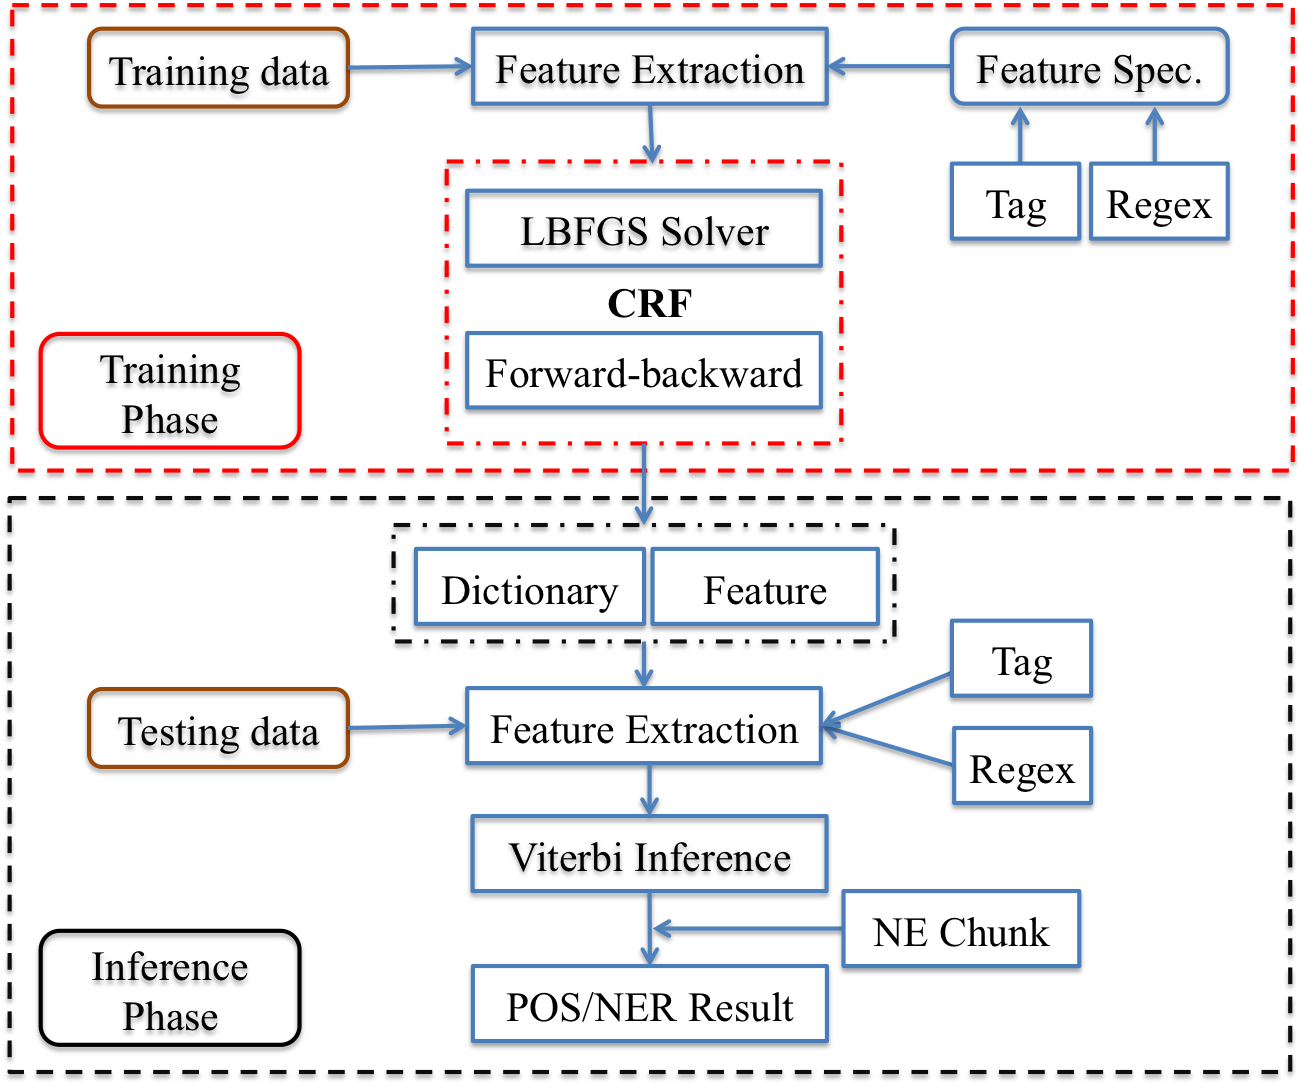
\includegraphics[height=15em]{system.png}
\end{center}

\subsection{Part-of-speech Tagging}
Part-of-speech tagging, also called grammatical tagging or word-category disambiguation is the process of assigning 
a part of speech to each word in a sentence. POS has been widely used in information retrieval and text to speech. 
There are two distinct methods for 
POS task: rule-based and stochastic.
In rule-based method, large collection of rules are defined to indentify the tag. Stochastic method is based on 
probabilistic graphic models such as hidden markov models and conditional random fields. In practice, 
conditional random fields are approved to achieve the state of art accuracy.

\subsubsection{Feature Extraction}
The Feature Extraction module provides functionality for basic text-analysis
tasks such as part-of-speech (POS) tagging and named-entity resolution.
At present, six feature types are implemented.
\begin{itemize}
\item Edge Feature: transition feature that encodes the transition feature weight from current label to next label.
\item Start Feature: fired when the current token is the first token in a sentence.
\item End Feature: fired when the current token is the last token in a sentence.
\item Word Feature: fired when the current token is observed in the trained dictionary.
\item Unknown Feature: fired when the current token is not observed in the trained dictionary for at least certain times.
\item Regex Feature: fired when the current token can be matched by the regular expression.
\end{itemize}

Advantages of extracting features using SQL statements:
\begin{itemize}
\item [$\star$] Decoupling the feature extraction and other code.
\item [$\star$] Compared with procedure language, SQL is much more easier to understand.
\item [$\star$] Storing all the features in tables avoids recomputing of features over iterations. It also boosts the performance.
\item [$\star$] SQL is naivelly paralleled.
\end{itemize}

\begin{itemize}
\item $SQL_1$:\\
\begin{lstlisting}[language=SQL,gobble=4]
    SELECT doc2.start_pos, doc2.doc_id, 'E.', ARRAY[doc1.label, doc2.label]
    FROM   segmenttbl doc1, segmenttbl doc2
    WHERE  doc1.doc_id = doc2.doc_id AND doc1.start_pos+1 = doc2.start_pos
\end{lstlisting}

\item $SQL_2$:\\
\begin{lstlisting}[language=SQL,gobble=4]
    SELECT start_pos, doc_id, 'R_' || name, ARRAY[-1, label]
    FROM  regextbl, segmenttbl
    WHERE seg_text ~ pattern
\end{lstlisting}
\end{itemize}

\paragraph{Build the feature dictionary and assign each feature with a unique feature id}
\begin{itemize}
\item $SQL_3$\\ 
\begin{lstlisting}[language=SQL,gobble=4]
    INSERT INTO tmp_featureset(f_name, feature) 
    SELECT DISTINCT f_name, feature
    FROM   tmp1_feature;
    INSERT INTO featureset(f_index, f_name, feature) 
    SELECT nextval('seq')-1, f_name, feature
    FROM   tmp_featureset;
\end{lstlisting}
\end{itemize}

\paragraph{Generate sparse\_r table}
\begin{itemize}
\item $SQL_3$\\ 
\begin{lstlisting}[language=SQL,gobble=4]
    INSERT INTO rtbl(start_pos,doc_id,feature)
    SELECT start_pos, doc_id, array_cat(fset.feature, 
			ARRAY[f_index,start_pos, 
			CASE WHEN tmp1_feature.feature = fset.feature THEN 1
			ELSE 0 END] )
    FROM   tmp1_feature, featureset fset
    WHERE  tmp1_feature.f_name = fset.f_name AND fset.f_name <> 'E.';
\end{lstlisting}
\end{itemize}


\subsubsection{Parallel Linear-chain CRF Training}

\paragraph{LBFGS Convex Optimization}
The limited-memory BFGS(L-BFGS) is the limited memory variation of the Broyden-Fletcher-Goldfarb-Shanno(BFGS) algorithm which
is the state of art of large scale non constraint convex optimization method.
We translate the in-memory Java implementation to C++ in-database implementation using Eigen support.
Eigen vector and Eigen matrix are used instead of the plain one dimentional and two dimentional arrays.
In the Java in-memory implementation, it defines many static variables defined and shared between the interations.
However, in the MADlib implementation, we define these variables in the state object.
Before each iteration of L-BFGS optimization, we need to initialize the L-BFGS with the current state object. 
At the end of each iteration, we need to dump the updated variables to the database state for next iteration.

\begin{lstlisting}[language=SQL,gobble=4]
    select crf_train_data('/path/to/trainingdataset')
\end{lstlisting}

\begin{lstlisting}[language=SQL,gobble=4]
    select crf_train_fgen('train_segmenttbl', 'crf_regex','crf_dictionary', 
    'featuretbl','crf_feature_dic')
\end{lstlisting}

\begin{lstlisting}[language=SQL,gobble=4]
    select lincrf('featuretbl','spars_r','dense_m','sparse_m','f_size',45, 
    'crf_feature_dic','crf_feature',20)
\end{lstlisting}

\subsubsection{Parallel Linear-chain CRF Inference}
 The Viterbi algorithm is to find the top-k most likely labelings of a document 
for CRF models. 
We chose to implement a Python UDF that uses iterations to drive the Viterbi inference. 
In Greenplum, Viterbi can be run in parallel over different subsets 
of the document on a multi-core machine.

The $vcrf\_top\_label$ is implemented sequentially and each function call will finish labeling of one document. 
The inference is paralledl in the level of document. We use a SQL statment to drive the inference of all documents.
So, the CRF inference is naivelly parallel. 
\begin{lstlisting}[language=SQL,gobble=4]
        SELECT doc_id, vcrf_top1_label(mfactors.score, rfactors.score)
        FROM   mfactors,rfactors
\end{lstlisting}

\paragraph{Inference}
\begin{lstlisting}[language=SQL,gobble=4]
    select crf_test_data('/path/to/testingdataset')
\end{lstlisting}

\begin{lstlisting}[language=SQL,gobble=4]
    select crf_test_fgen('test_segmenttbl',
    'crf_dictionary','crf_label','crf_regex',
    'crf_feature','viterbi_mtbl','viterbi_rtbl')
\end{lstlisting}

\begin{lstlisting}[language=SQL,gobble=4]
    select vcrf_label('test_segmenttbl', 
    'viterbi_mtbl','viterbi_rtbl',
    'crf_label','extraction')
\end{lstlisting}


\subsection{Entity Detection}

\subsection{Layout}
\label{ssec:layout}

Format manuscripts two columns to a page, in the manner these
instructions are formatted. The exact dimensions for a page on US-letter
paper are:

\begin{itemize}
\item Left and right margins: 1 inch
\item Top margin: 1 inch
\item Bottom margin: 1 inch
\item Column width: 3.15 inches
\item Column height: 9 inches
\item Gap between columns: 0.2 inches
\end{itemize}

\noindent Papers should not be submitted on any other paper size. Exceptionally,
authors for whom it is \emph{impossible} to format on US-Letter paper,
may format for \emph{A4} paper. In this case, they should keep the \emph{top}
and \emph{left} margins as given above, use the same column width,
height and gap, and modify the bottom and right margins as necessary.
Note that the text will no longer be centered.

\subsection{The First Page}
\label{ssec:first}

Center the title, author's name(s) and affiliation(s) across both
columns (or, in the case of initial submission, space for the names). 
Do not use footnotes for affiliations.  Do not include the
paper ID number assigned during the submission process. 
Use the two-column format only when you begin the abstract.

{\bf Title}: Place the title centered at the top of the first page, in
a 15 point bold font.  (For a complete guide to font sizes and styles, see Table~\ref{font-table}.)
Long title should be typed on two lines without
a blank line intervening. Approximately, put the title at 1in from the
top of the page, followed by a blank line, then the author's names(s),
and the affiliation on the following line.  Do not use only initials
for given names (middle initials are allowed). Do not format surnames
in all capitals (e.g., ``Bangalore,'' not ``BANGALORE'').  The affiliation should
contain the author's complete address, and if possible an electronic
mail address. Leave about 0.75in between the affiliation and the body
of the first page.

{\bf Abstract}: Type the abstract at the beginning of the first
column.  The width of the abstract text should be smaller than the
width of the columns for the text in the body of the paper by about
0.25in on each side.  Center the word {\bf Abstract} in a 12 point
bold font above the body of the abstract. The abstract should be a
concise summary of the general thesis and conclusions of the paper.
It should be no longer than 200 words.  The abstract text should be in 10 point font.

{\bf Text}: Begin typing the main body of the text immediately after
the abstract, observing the two-column format as shown in 
the present document.  Do not include page numbers.

{\bf Indent} when starting a new paragraph. For reasons of uniformity,
use Adobe's {\bf Times Roman} fonts, with 11 points for text and 
subsection headings, 12 points for section headings and 15 points for
the title.  If Times Roman is unavailable, use {\bf Computer Modern
  Roman} (\LaTeX2e{}'s default; see section \ref{sect:pdf} above).
Note that the latter is about 10\% less dense than Adobe's Times Roman
font.

\section{Performance Evaluation}
\label{sec:length}

\subsection{Scalability}
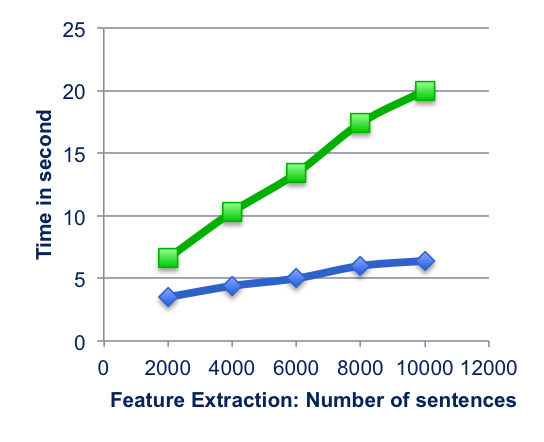
\includegraphics[height=9.9em,width=10em]{extraction.png}
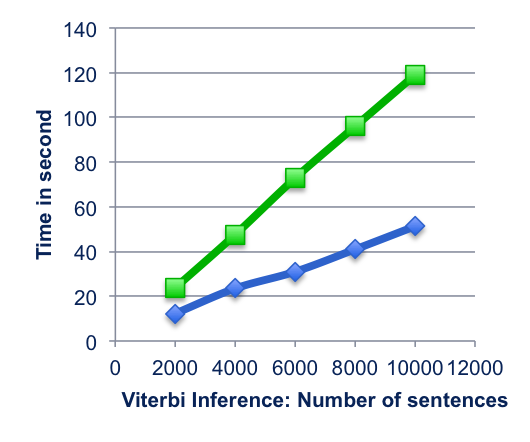
\includegraphics[height=9.9em,width=10em]{viterbi.png}

\subsection{Comparisons with the State of Art}
Compared with PCRF, CRF++

\section{User Case: Tweet Analysis}
\label{sec:blind}

As the reviewing will be blind, the paper must not include the authors' names and affiliations. Furthermore, self-references that reveal the author's identity, e.g., ``We previously showed (Smith, 1991) ...'' must be avoided. Instead, use citations such as ``Smith previously showed (Smith, 1991) ...'' Papers that do not conform to these requirements will be rejected without review. In addition, please do not post your submissions on the web until after the review process is complete.

\section*{Acknowledgments}
Christan Grant is funded by a National
Science Foundation Graduate Research Fellowship under Grant No. DGE-0802270.
This work was supported by a gift from EMC Greenplum.

\begin{thebibliography}{}

\bibitem[\protect\citename{Aho and Ullman}1972]{Aho:72}
Alfred~V. Aho and Jeffrey~D. Ullman.
\newblock 1972.
\newblock {\em The Theory of Parsing, Translation and Compiling}, volume~1.
\newblock Prentice-{Hall}, Englewood Cliffs, NJ.

\bibitem[\protect\citename{{American Psychological Association}}1983]{APA:83}
{American Psychological Association}.
\newblock 1983.
\newblock {\em Publications Manual}.
\newblock American Psychological Association, Washington, DC.

\bibitem[\protect\citename{{Association for Computing Machinery}}1983]{ACM:83}
{Association for Computing Machinery}.
\newblock 1983.
\newblock {\em Computing Reviews}, 24(11):503--512.

\bibitem[\protect\citename{Chandra \bgroup et al.\egroup }1981]{Chandra:81}
Ashok~K. Chandra, Dexter~C. Kozen, and Larry~J. Stockmeyer.
\newblock 1981.
\newblock Alternation.
\newblock {\em Journal of the Association for Computing Machinery},
  28(1):114--133.

\bibitem[\protect\citename{Gusfield}1997]{Gusfield:97}
Dan Gusfield.
\newblock 1997.
\newblock {\em Algorithms on Strings, Trees and Sequences}.
\newblock Cambridge University Press, Cambridge, UK.

\end{thebibliography}

\end{document}
